
\chapter{Case and artificial language evolution}
\section{Introduction}
The more than 6.000 languages in the world each have their unique way of offering their speakers an astonishing range of expressivity. We can just as easily engage in hair-splitting philosophical debates as we can start gossiping about as soon as somebody leaves the room. At the heart of the grammar that allows us to communicate all these complex meanings lies the way in which relations between words are organized. If you want to hear about juicy facts such as who kissed whom, grammar can help you finding out using various strategies such as word order\is{word order}, verbal agreement\is{agreement} and case marking\is{case!case marking}.

Among all the possible strategies employed by language users, only few have seduced linguists so skillfully as grammatical case has done. Ever since P\={a}\d{n}ini(4th Century BC), case has claimed a central role in linguistic theory and continues to do so today. However, despite centuries worth of research, case has yet to reveal its most important secrets, as can be gleaned from the many recent monographs \citep{blake94case,butt06theories}, collections \citep{kulikov06casebook,barddal09casebook,malchukov09case} and projects (``Case and thematic relations'', \citealp{davidse96functional}; PIONEER, \citealp{amberber05competition}; ``Indo-European Case and Argument Structure in a Typological Perspective'', \citealp{barddal09case}). 
Among the many open questions, the following two are explored in this book:

\begin{enumerate}
\item Why do some languages evolve a case system?
\item How can a population self-organize a case system?
\end{enumerate}

Both challenges have proven to be problematic and even controversial in the literature on case. The first question is answered differently by each linguistic theory -- if answered at all. The second one has largely been out of reach of linguists due to insufficient historical data, which makes that changes in a language can often only be detected once that change has already propagated and become acceptable in a population \citep[34--35]{croft91syntactic}.

This book proposes that case categories are {\em culturally} constructed (as opposed to being innate), and that a case system may emerge spontaneously as language users try to optimize their communicative success in locally situated interactions while at the same time minimizing the cognitive resources required to do so. 

The validity of this hypothesis is demonstrated through agent-based modeling -- a research methodology that is well-established in fields such as biology and economics, but which is still relatively unknown in linguistics. One reason is that experiments in artificial language evolution have so far mainly focused on simple one-to-one mappings between meaning and form, whereas all natural language systems are highly complex and ambiguous phenomena. As the experiments in this book will show, however, it is perfectly feasible to tackle such intricate phenomena as well if we use more sophisticated tools for handling linguistic representations and processing. 

\section{Case and the grammar square}
\label{s:grammar-square}
\subsection{Overview}  
Before delving into methodological issues, however, let us first look at the empirical domain that needs to be modeled in order to have a clear appreciation of the complexity of case systems and the problem of ``argument realization'' (i.e. the relation between event structure and its morphosyntactic realization in language).

\subsection{The functions of case systems}
\label{s:case-functions}

Most case systems are used as a device for marking what the role of a participant is in a particular event. Consider the following example from Turkish\is{Turkish}:

\label{e:case1}
\ea
\gll Mehmet adam-a elma-lar-ı ver-di. \\
	Mehmet.{\nom} man-{\dat} apple-{\pl}-{\acc} give-{\pst}-3{\sg} \\
\glt `Mehmet gave the apples to the man.' \citep[1, example 1]{blake94case}
\z

The case marker\is{case!case marking}s make it clear to the hearer that Mehmet was the giver of the apples, not the recipient\is{semantic role!recipient}. Marking the roles of participants in an event has some serious advantages: it allows the hearer to interpret the utterance correctly without actually observing the scene (i.e. ``displacement\is{displacement}'' becomes possible) because it rules out ambiguities, and it reduces the semantic complexity of parsing because the hearer does not have to infer who was the giver and who was the receiver from other contextual cues. So one of the basic functions of case marking\is{case!case marking} is {\bfseries to indicate event structure\is{event structure}}.

Secondly, case marker\is{case!case marking}s are also used {\bfseries for packaging information structure\is{information structure}}. In example \ref{e:case1}, the suffix {\em -ı} not only marks the accusative\is{case!accusative} case, but it also indicates that the apples are ``specific'' (as opposed to undetermined). Many languages also exploit case marker\is{case!case marking}s for marking the topic and focus of an utterance, for marking new vs. given information, and so on.

Finally, case marking\is{case!case marking} can be used for indicating various other grammatical distinctions such as number\is{number} and gender\is{gender}, as shown here for German\is{German}:

\ea
\gll ein klein-er Man \\
a little-\textsc{m.sg} man \\
\glt `a little man' \\
\z

\ea
\gll drei klein-e Frau-en \\ 
three little-{\pl} woman-\textsc{f.pl} \\
\glt `three little women' \\
\z

This book focuses on the first function of case systems: indicating event structure. More specifically, it reports on experiments in artificial language evolution that show how a primitive case system may emerge in a multi-agent population. In order for the experiments to have any scientific value, they must be compatible with what is known about the evolution of real-life case systems, which I will summarize in the following sections.

\subsection{Stage I: no marking}
\label{s:stage1}

Many languages do not have a case system at all, but rather employ a different strategy such as word order (e.g. English). There are even languages that hardly use any marking whatsoever for indicating ``who did what to whom'' to the hearer. For instance, the language Lisu generally does not mark event structure. \citeauthor{li76subject} (1976; quoted from Palmer \citeyear{palmer94grammatical}:23) give the following two examples:

\eal
\ex[]{
\label{e:lisu1}
\gll làma nya ánà khù-a. \\
tigers \textsc{top} dog bite-\textsc{decl} \\
\glt `Tigers bite dogs.' / `Dogs bite tigers.'
}
\ex[]{
\label{e:lisu2}
\gll ánà x{\textschwa} làma  khù-a. \\
dog \textsc{new top} tigers bite-\textsc{decl} \\
\glt `Tigers bite dogs.' / `Dogs bite tigers.'
}
\zl

In both sentences, there is only a topic marker (``known topic'' versus ``new topic''), but the correct reading depends on the context in which the sentence was uttered. Another example is Riau Indonesian \citep{gil08how}, which only marks event structure in extremely rare cases. While such examples seem odd for speakers of most other languages, \citet[23]{palmer94grammatical} notes that even English does not always mark event structure. For example, the famous phrase {\em the shooting of the hunters} does not indicate whether the hunters did the shooting or whether they got shot themselves.

\begin{figure}[t]
\centerline{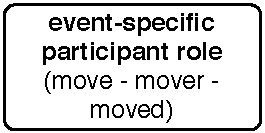
\includegraphics[scale=0.6]{chap-introduction/figs/stage1}}
    \is{formation}
    \caption[Formation of case markers: stage II]{In the first stage, the experiments start with a lexicon but without any grammar. The lexicon may contain words such as {\em move}, whose event structure may include participant roles such as ``mover'' (i.e. the one who did the moving) and ``moved'' (i.e. the thing that is being moved). However, the language has no means of marking those participant roles explicitly, hence the hearer has to infer the intended interpretation from the context.}
      \label{f:stage1}
\end{figure}

The experiments in this book therefore start from the point where a population of language users have already evolved a lexicon, but {\bfseries no grammar yet} (see \figref{f:stage1}). This point of departure is not only justified by the empirical observation that new case markers evolve from existing lexical items (see further below), but also by the fact that experiments on artificial language evolution have already shown how vocabularies may emerge in a population of grounded embodied agents \citep[e.g.][]{steels96emergent, steels96selforganizing, steels97selforganizing}. In this way we can better isolate the features that are hypothesized to be formed in the experiments. Of course, once the dynamics of these experiments are better understood, a series of integrated experiments must be carried out to confirm the results.

\subsection{Stage II: specific marking}
\label{s:stage2}

\largerpage
Attested examples of the emergence\is{emergence} of modern case marker\is{case!case marking}s show that they are recruited from existing lexical items and that they start out in very restricted use scenarios. \citet[chapter 6]{blake94case} gives examples of how verbs, noun\is{noun}s and even adverb\is{adverb}ial particles can develop into case marker\is{case!case marking}s. Blake writes that a predicate like COME is a two-place predicate implying a ``comer'' and a ``destination''. A predicate like LEAVE mirrors this implication by having a ``leaver'' and a ``source\is{semantic role!source}''. A predicate like FLY, however, only implies a ``flier''. If speakers then wish to produce utterances such as {\em he flew to/from Bangkok}, pairs of predicates can be used. Blake gives the following examples from Thai\is{Thai}:

\eal
\label{e:thai}
\ex[]{
\gll th\^{a}n cà bin maa krungth\^{e}ep \\
he will fly come Bangkok \\
\glt `He will fly to Bangkok.'
}
\ex[]{
\gll th\^{a}n cà bin càak krungth\^{e}ep \\
he will fly leave Bangkok \\
\glt `He will fly from Bangkok.'
}
\hspace{0.2cm}\citep[163--164]{blake94case}
\zl

\begin{figure}[b]
\centerline{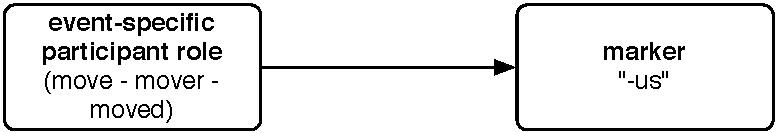
\includegraphics[scale=0.6]{chap-introduction/figs/stage2}}
  \caption[Formation\is{formation} of case markers: stage II]{In the second stage, a specific marker\is{case!case marking} arises in order to solve a communicative problem. In natural languages, this marker\is{case!case marking} is often a lexical item which is recruited for a new use. In the experiments, this stage involves the invention of a new marker\is{case!case marking}.}
   \label{f:stage2}
\end{figure}

Such languages are known as ``serial verb language\is{serial verb} languages''. The second verb is (usually) non-finite\is{finiteness} and cannot be marked for tense\is{tense}, aspect\is{aspect} or mood\is{modality} independently of the first verb, and it takes no expressed subject\is{syntactic role!subject} or it implies the same subject\is{syntactic role!subject} as that of the first verb. Blake writes that functionally speaking, these second verbs are equivalent to preposition\is{preposition}s. Serial verb language\is{serial verb language\is{serial verb}} constructions are in fact very frequent and their development into adposition\is{adposition}s and case marker\is{case!case marking}s has been widely attested, especially in the languages of West Africa, New Guinea, Southeast Asia and Oceania (ibid., at 163; also see \citealp{givon97introduction}, section 7, for more on serial verb language\is{serial verb} constructions and similar examples).

The recruitment and evolution\is{evolution!cultural evolution} of a lexical item into an adposition\is{adposition} and eventually a case marker\is{case!case marking} is a long and complex process. For reasons that I will explain later on in this book, this crucial step in grammaticalization\is{grammaticalization} is ``scaffold\is{scaffold}ed'' in the experiments. Rather than reusing\is{reuse} an existing lexical item in a more grammatical way, the artificial agents will be capable of inventing a new form which already acts as some kind of adposition\is{adposition} or verb-specific case marker\is{case!case marking}, as shown in \figref{f:stage2}. The experiments thus simplify stage II in order to focus first on the function of such marker\is{case!case marking}s and how they can be propagat\is{propagation}ed in a speech community\is{speech population}. It is needless to say, however, that this part of the grammaticalization\is{grammaticalization} chain remains on the research agenda for future experiments and first steps towards grammaticalization\is{grammaticalization} of existing lexical elements have already been taken by \citet{wellens08flexible}.

\subsection{Stage III: semantic roles}
\is{semantic role}
\label{s:stage3}

When verb-specific case markers propagate successfully in a speech community, they often extend their coverage to other verbs as well. To come back to example \ref{e:thai}, this would mean that {\em maa} `come' evolves from the marker\is{case!case marking} of the destination of a flight to a general allative\is{case!allative} case role (i.e. the destination of motion events). Extension of the use of a marker\is{case!case marking} would in this case be {\em semantically motivat\is{semantic motivation}ed} and can occur by analog\is{analogy}ical reasoning over events. This is also the strategy that is employed in the experiments. 

\figref{f:stage3} illustrates the new mapping between meaning and form when case markers become generalized semantic markers. Instead of directly mapping a particular participant role (e.g. the ``mover'') onto a case marker, a {\bfseries semantic role} (such as Agent) mediates between this mapping.

Since case marker\is{case!case marking}s in natural languages usually carry more than one function, it is hard to say what the semantic role\is{semantic role}s are that underlie a syntactic pattern. We can however look at ``agnating structures'' \citep{gleason65linguistics}. Agnation\is{agnation} illustrates a structural relationship between two grammatical constructions which have the same (major) lexical items, but different syntactic structures. If the alternation between these two structures is recurrent for groups of constructions, then this can be seen as a pattern in the language. An example of agnating\is{agnation} structures is the alternation between the English\is{English} ditransitive\is{ditransitive clause} (as in {\em I gave him a book}) and its preposition\is{preposition}al counterpart (as in {\em I gave the book to him}). 

Differences in the semantic categorization of verbs can come to surface if small but regular variation\is{variation}s show up between these agnating\is{agnation} structures. Compare the groups of agnating\is{agnation} structures in the following examples:

\begin{figure}[t]
\centerline{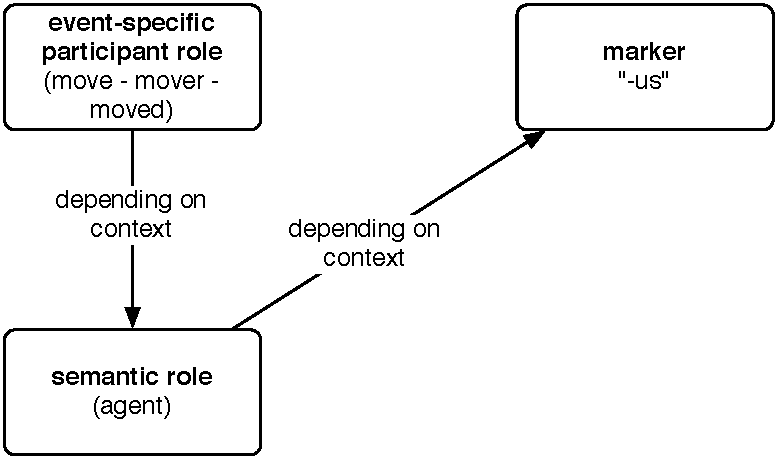
\includegraphics[scale=0.6]{chap-introduction/figs/stage3}}
  \caption[Formation\is{formation} of case markers: stage III]{Specific marker\is{case!case marking}s may get exten\is{extension}ded through analog\is{analogy}y in stage III. They now start to act as semantic role\is{semantic role}s.}
   \label{f:stage3}
\end{figure}

\ea
\label{e:agnate1}
\begin{tabbing}
I gave him a book. \hspace{2cm} \= I gave the book to him.
\\ I sent him a letter. \> I sent the letter to him.
\end{tabbing}
\z
\ea
\label{e:agnate2}
\begin{tabbing}
I baked him a cake. \hspace{1,85cm} \= I baked a cake for you.
\\I bought him a present. \> I bought a present for him.
\end{tabbing}
\z

Both groups of verbs can occur in the ditransitive\is{ditransitive clause} construction, but they select a different preposition\is{preposition} in the agnating\is{agnation} preposition\is{preposition}al construction. The choice for either {\em to} or {\em for} is semantically motivat\is{semantic motivation}ed: the verbs listed in example \ref{e:agnate1} entail\is{entailment} an {\em actual} transfer of the direct object\is{syntactic role!object} (= recipient), whereas the verbs in \REF{e:agnate2} indicate that there is an {\em intended} transfer (= beneficiary). This is confirmed in the fact that sentences such as {\em ?I gave him a book, but he refused it} feel awkward, whereas sentences such as {\em I baked him a cake, but he refused it} are perfectly acceptab\is{acceptability}le. So it seems that both groups of verbs belong to different subclasses.

The exten\is{extension}sion of specific marker\is{case!case marking}s to semantic role\is{semantic role}s is useful for communication in several ways. First of all, semantic role\is{semantic role}s increase the potential for generalization in a language: by exten\is{extension}ding the functionality of a semantic role\is{semantic role}, there is a higher chance that it will be reuse\is{reuse}d for categorizing new and similar participant role\is{participant role}s as well. Instead of having to negotiat\is{negotiation}e a different marker\is{case!case marking} for each new instance, speakers of a language can thus make a semantically motivat\is{semantic motivation}ed innovat\is{innovation}ion which increases the chance that the hearer will understand the speaker's intention. Second, and related to the first point, semantic role\is{semantic role}s increase the expressiveness\is{expressiveness} of a language because they allow speakers to profile different aspects of the same event. For example, semantic role\is{semantic role}s can focus on the relation between an agent\is{semantic role!agent} and a patient\is{semantic role!patient} as in {\em he broke the window}, but also profile exclusively the resulting state\is{aspect!state} of one of the participants as in {\em the window was broken}. Finally, semantic role\is{semantic role}s can significantly reduce the inventory size by grouping together larger classes of verbs.

The model proposed in this book predicts that the convention\is{convention}alization of a mapping between verb-specific arguments and semantic role\is{semantic role}s (even though semantically motivat\is{semantic motivation}ed) is neither a determined nor a straightforward one. The choice depends on the convention\is{convention}s that are already present in the language, on a speaker's previous experience, frequency\is{frequency}, etc. Moreover, the model predicts that there will be several varieties in the population\is{speech population} which compete with each other for becoming the dominant semantic role\is{semantic role} of a particular argument. Thus we can expect that languages come up with very divergent classifications. For example, Italian\is{Italian} features dative\is{case!dative} subject\is{syntactic role!subject}s with verbs such as {\em like} \citep[27]{palmer94grammatical}, whereas English doesn't:

\ea
\gll Gli piacciono le ciliege. \\
they.{\dat} like \textsc{det} cherries \\
\glt `They like cherries.'  \\
\z


Linking similar events can also be reversed from language to language. For example, when French\is{French} speakers want to say {\em I miss you}, they literally say something like `you are missing to me':

\ea
\gll Tu me manque-s. \\
you me miss-2{\sg}.{\prs} \\
\glt `I miss you.' \\
\z


So semantic role\is{semantic role}s seem to be language-specific, which fits our assumption\is{assumption} that they have to be constructed and learned. But once they become part of a language, are they an affair of `take it or leave it', or is it possible that the same verb-specific participant role\is{participant role} can be mapped onto multiple semantic role\is{semantic role}s? The answer seems to be that this mapping too is indirect and dependent on the context. For example, the `sneezer' in {\em he sneezes} seems to be a patient\is{semantic role!patient}, whereas it is (also) a causer\is{semantic role!causer} in {\em he sneezed the napkin off the table}. All the above observations are reflected in \figref{f:stage3} and more evidence is provided in the next chapter.

\subsection{Stage IV: syntactic roles}
\is{syntactic role}
\label{s:stage4}

\begin{figure}[t]
\centerline{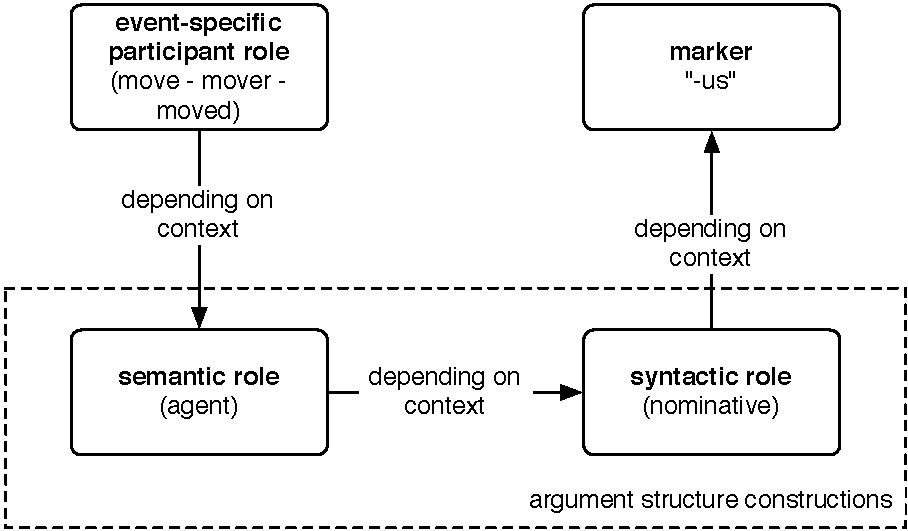
\includegraphics[scale=0.6]{chap-introduction/figs/case-quadrant}}
  \caption[Formation\is{formation} of case markers: stage IV]{In the next step, even more abstraction\is{abstraction}s occur through syntactic role\is{syntactic role}s. The mapping between semantic role\is{semantic role}s and grammatical cases is hypothesized to be handled by \is{event structure}\is{construction!argument structure construction}argument structure constructions which can combine several semantic role\is{semantic role}s into a larger pattern.}
   \label{f:stage4}
\end{figure}

Languages typically have thousands of verbs and semantic roles. However, case languages tend to have streamlined case systems with only a dozen cases or less. As \citet{croft91syntactic} states

\begin{quote}
surface case marking\is{case!case marking} imposes structure on thematic relations to an even more abstract degree than verb roots impose structure on the human experience of events.  \citep[158--159]{croft91syntactic}
\end{quote}

We know that a case marker has evolved into a {\em syntactic} marker once it can be dissociated from a particular semantic role \citep[2--3]{givon97introduction}. For instance, the German nominative case can be used for covering virtually all semantic roles of the language. 

\figref{f:stage4} shows an updated mapping between event structure meaning and its surface form, which is now mediated by an abstract and hidden layer of semantic and syntactic categories. I will from now on refer to this picture as the {\bfseries grammar square}. Each mapping in the square can vary according to the communicative and linguistic circumstances, so the relation between a participant role\is{participant role} and its morphosyntactic realization is multilayered and indirect.

The picture presented here however has the danger that case marker\is{case!case marking}s are considered in isolation, whereas they can only be understood in relation to the other parts of the pattern in which they occur. Indeed, the mapping of semantic role\is{semantic role}s onto syntactic role\is{syntactic role}s (and vice versa) is hypothesized to be taken care of by \is{event structure}\is{construction!argument structure construction}{\bfseries argument structure constructions} \citep{goldberg95construction}. These constructions may be schematic, verb-class-specific\is{construction!verb-class-specific construction} or even verb-specific. I will come back to this point in the next Chapters that introduce the formalization of such constructions.

\subsection{Further developments}
\label{s:case-markers}

\largerpage
Stages I--IV described the possible evolutionary pathway of a case marker\is{case!case marking} which resulted in an inflection\is{inflection}al category that groups together various semantically related roles. This is also the endpoint of the experiments described in this book because they focus only on case marking\is{case!case marking} as a way to express event structure\is{event structure} in a grammatical way. There are, however, other functions which may be performed by case marker\is{case!case marking}s such as packaging information structure\is{information structure}, marking perspectiv\is{linguistic perspective}ization and other grammatical distinctions such as gender\is{gender} and number\is{number} (as argued in \sectref{s:case-functions}). Especially information structure\is{information structure} seems to be the most important pressure for case marker\is{case!case marking}s to exten\is{extension}d their coverage and become even more dissociat\is{dissociation}ed from their previous meaning.

Finally, case marker\is{case!case marking}s eventually decline and even whole grammatical systems\is{case!case system} of case may get lost and replaced by other grammatical devices. This is apparent in the (almost) complete loss of case marking\is{case!case marking} in languages such as English\is{English}, French\is{French} and Dutch\is{Dutch}, which replaced it with word order\is{word order} constraints. Individual case marker\is{case!case marking}s may disappear because they are ``merged'' with another case such as the merger of the instrumental\is{case!instrumental} and locative\is{case!locative} case in Middle Indo-Aryan\is{Indo-Aryan} \citep[176]{blake94case}. Whereas merger seems to be relatively common in the life cycle of case systems\is{case!case system}, case split\is{case!case split} is quite rare. Merger of case marker\is{case!case marking}s means that the case system\is{case!case system} is reduced unless new members are recruited. With the loss of cases and further developments in the grammaticalization\is{grammaticalization} of case marker\is{case!case marking}s, the different cases of a language may become insufficiently differentiated from each other. This allows other strategies, such as word order\is{word order} complemented with preposition\is{preposition}s in English\is{English}, to become more popular and eventually the new convention\is{convention}s of a language. The decline of entrench\is{entrenchment}ed and convention\is{convention}alized grammatical units falls beyond the scope of this book.

\section{Modeling language evolution}
\label{s:models}

\subsection{Overview}
The experiments reported in this book are models of {\em artificial language evolution}, in which computational and mathematical models and robotic experiments are used for evolving (new) artificial languages that have similar properties as found in natural languages. As such, the methodology provides possible and operational explanations for those properties. Experiments typically involve a {\em population of artificial language users} (henceforth called {\em agents}) that engage with each other in communicative interactions. 

\subsection{Three models of artificial language evolution}

There is a wide consensus in the field that language has evolved because there is a {\em selectionist} system underlying it. Despite this consensus, there is disagreement on how linguistic variation and hence the potential for change is caused, and which selectionist pressures are operating to retain a particular variation in a language. There are basically three different perspectives based on genetic evolution, cultural transmission, and problem-solving respectively.

\begin{figure}[t]
\centerline{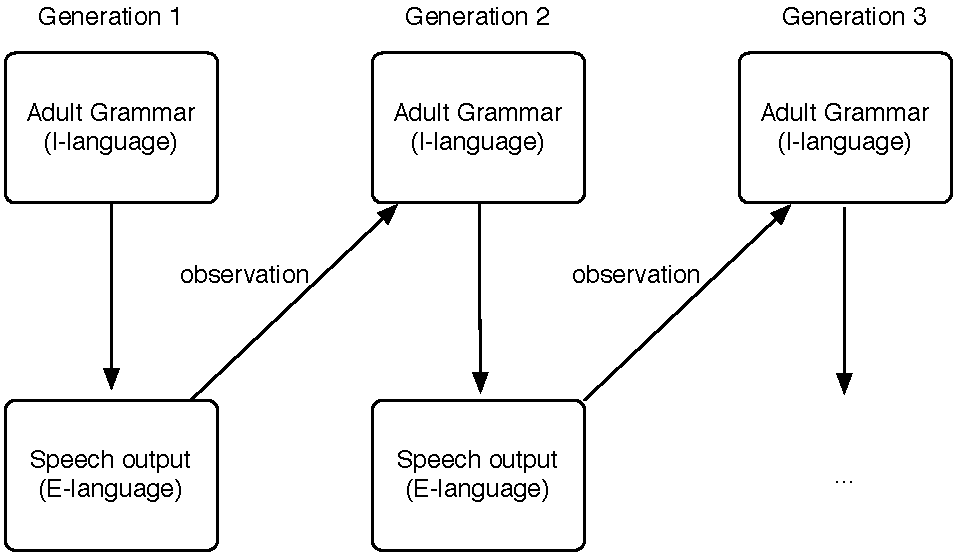
\includegraphics[scale=0.55]{chap-introduction/figs/childbased}}
  \caption[Child-based language change\is{language change}]{Iterated learning models assume that languages evolve because children are faced with a learning bottleneck when observing and reconstructing the language of the previous generation.}
   \label{f:child-based}
\end{figure}

Models of genetic evolution \citep[e.g.][]{briscoe00grammatical, nowak01evolution} investigate the biological evolution of the {\em language faculty} (i.e. our ability to acquire and use language). These models put the selectionist pressure at the level of fitness (i.e. the ability to survive and reproduce), which is assumed to be directly related to communicative success. Agents are endowed with an artificial genome that determines their communicative behavior. Depending on how much of language is assumed to be innate, the genome may include which concepts can be employed by the agents for structuring their world, which types of categories are to be used, and so on. Potential innovation takes place when this genome is transmitted from parents to children. Because genome copying involves crossover\is{crossover} and possibly mutation\is{mutation}, variation\is{variation} is inevitable, and some of it will lead to higher or lower success.

\is{Iterated Learning Model (ILM)} Iterated Learning Models (ILM, \citealt{brighton05cultural, kirby01spontaneous, kirby02emergence, kirby04from, smith03iterated}) investigate what happens when language is culturally transmitted from one generation to the next without any interference from functional pressures, as illustrated in \figref{f:child-based}. Each cycle, an adult generation (typically represented by a single agent) produces speech output based on its internal grammar, which is observed by a new generation (also typically a single agent) for reconstructing the language. The model assumes that there is a learning bottleneck (i.e. the child cannot observe all utterances in the language), hence the learner agent may overgeneralize the input based on innate learning biases. When the adult agent ``dies'' and is replaced by the child, the mistakes in learning become the new convention and the language changes. The ILM shows strong affinity for child-based theories of language change as found in generative linguistics \citep{king69historical}.

The third class of models views the task of building and negotiat\is{negotiation}ing a communication system as a kind of problem-solving\is{problem-solving} process. Agents try to achieve a communicative goal with maximal success and minimal effort. This problem-solving\is{problem-solving} process is definitely not a rational but an intuitive one that is seldom accessible to conscious inspection. It is not an individualistic problem-solving\is{problem-solving} process either, but a collective one, in which different individuals participate as peers. According to this view a communication system is built up in a step by step fashion driven by needs and failures in communication, and it employs a large battery of strategies and cognitive mechanisms which are not specific to language but appear in many other kinds of cognitive tasks, such as tool design\is{tool design} or navigation\is{navigation}. Recent experiments by \citet{galantucci05experimental} on the emergence\is{emergence} of communication in human subject\is{syntactic role!subject}s provide good illustrations of these problem-solving\is{problem-solving} processes in action. Variation and innovat\is{innovation}ion in problem-solving\is{problem-solving} models are common because each individual not only tries to converge to the shared communication system, but can also contribute innovat\is{innovation}ions to it. In fact the main challenge is rather to explain how agreement between individuals and thus a globally shared population\is{speech population} language can ever arise. This approach to language evolution\is{evolution!cultural evolution} is closely related to cognitive-functional\is{cognitive-functional approach} theories of language and utterance-based\is{selection!utterance-based selection} models of linguistic change \citep{croft00explaining, croft05relevance}.

The three models are of course not mutually exclusive: it is clear that the models of cultural evolution\is{evolution!cultural evolution} expect a rich cognitive-linguistic system, which can only be explained through the genetic endowment of the agents. Similarly, problem-solving\is{problem-solving} models can be modeled using a generation turnover as well \citep{vogt07group}. However, one particular advantage of the problem-solving approach is that it attempts to explain as many linguistic phenomena as possible in terms of functional and communicative pressures. This means that innate mechanisms are only used as a last resort, which arguably avoids putting all the explanatory burden on the shoulders of biology. This book therefore subscribes to the problem-solving approach.

\subsection{The do's and don'ts of artificial language evolution}
\is{artificial language evolution}
\label{s:methodology}

The question of the origins and evolution of language is notoriously difficult because there are no fossil traces or written accounts left of the first languages, and there are no data available about the biological changes that enabled language. These facts have led \citet{kirby03language} to pose the provocative question: is language evolution\is{evolution!cultural evolution} the hardest problem in science?

Without attempting to answer that question, it actually {\em is} possible to come up with solid theories despite the lack of real-life data: in various other disciplines, such as the origins\is{origins} of the universe, significant advances are made using mathematical models and computational simulations. Another example is Artificial Life\is{Artificial Life} where computational models, robot\is{robot}ic experiments and biochemistry are used as techniques to develop artificial phenomena that may help to explain processes of evolution in natural phenomena.

{\bfseries (i) Creating natural language-like phenomena.} Let me start by debunking a myth about modeling language evolution that seems to be lingering in the minds of some people: computational simulations and robot\is{robot}ic experiments can never lead to the emergence\is{emergence} of an actual natural language like English\is{English} or Russian\is{Russian}. There are just too many factors that have shaped these languages and modeling them would require to model the entire state of every speaker and every interaction {\em ever}. The ``languages'' that emerge in this kind of experiments should thus not be {\em directly} linked to natural languages: they are novel artificial constructs and hence {\bfseries the methodology only offers a ``proof of concept'' of what results can be achieved within the specific set-up of a given experiment}. However, these constructs may be natural language{\em -like} and thus offer a possible and working hypothesis for how similar phenomena could have come about in natural languages.

Secondly, even in abstraction, we cannot model every aspect of language at once, just as it is impossible to perform controlled psycholinguistic experiments that take every detail about language processing into account. The key is therefore to pick a phenomenon observed in natural languages and try to isolate this feature into a controlled simulation or experiment. Focusing on smaller problems is standard practice in many scientific disciplines. As Stephen Hawkin writes in his {\em A Brief History of Time}:

\begin{quote}
It turns out to be very difficult to devise a theory of the universe all in one go. Instead, we break the problem up into bits and invent a number of partial theories. Each of these partial theories describes and predicts a certain limited class of observations, neglecting the effects of other quantities, or representing them by simple sets of numbers. It may be that this approach is completely wrong. If everything in the universe depends on everything else in a fundamental way, it might be impossible to get close to a full solution by investigating parts of the problem in isolation. Nevertheless, it is certainly the way we have made progress in the past. 
\\ \cite[12]{hawkin88brief}
\end{quote}

In problem-solving models of artificial language evolution\is{artificial language evolution}, the researcher therefore first chooses a topic of interest that is common to most if not all languages, such as tense\is{tense}, aspect\is{aspect} and mood\is{modality}. Investigating such a feature involves the following steps \citep{steels06how}:


\begin{enumerate}
\item The researcher selects a feature of language to investigate;
\item The researcher hypothesizes which set of cognitive mechanisms and external pressures are necessary for the emergence\is{emergence} of this feature:
\begin{enumerate}
\item These cognitive mechanisms are operationalized in the form of computational processes, and a population\is{speech population} of simulated or embodied agents is endowed with these mechanisms;
\item The external pressures are operationalized in the form of an interaction pattern embedded in a simulated or real world environment;
\end{enumerate}
\item Systematic computer simulations are performed demonstrating the impact of the proposed mechanisms. If possible, results should be compared between simulations {\em with} a proposed mechanism and simulations {\em without} this mechanism in order to show that it is not only a sufficient but also a necessary prerequisite for the emergent feature. 
\end{enumerate}

Even if the simulations show that the investigated feature only emerges if certain mechanisms are included, this still does not prove anything about similar features in natural languages because different evolutionary pathways are possible. However, the simulations then at least show one possibility and may provide an additional piece of the puzzle next to evidence from linguistics, archeology, biology and other fields.

{\bfseries (ii) Clarifying the scaffold\is{scaffold}s and assumption\is{assumption}s.} Computational simulations and robot\is{robot}ic experiments are at the same time blessed and cursed with the fact that every detail of the hypothesis has to be spelled out completely, otherwise the system does not work. ``Blessed'' because this may reveal effects of the hypothesis that were overlooked or not expected by the verb\is{verb}al theory; ``cursed'' because there is a danger of ``kludging'' something together to get the system off the ground. There is often a fine border between significant results and quirks resulting from a kludge, so it is crucial that it is crystal clear which features of the model are supposed to be ``emergent'' on the one hand, and which features are ``assumed'' or ``scaffold\is{scaffold}ed'' on the other.

Assumptions and scaffold\is{scaffold}s are unavoidable in computational simulations because it is simply impossible to explain everything at once. Drawing the line between what is ``assumed'' and what is ``scaffold\is{scaffold}ed'' is not always an easy decision. I define ``assumed features'' as those aspects of the simulations that we cannot explain using the methodology described here. One example is the assumption\is{assumption} that agents are social and cooperative beings that {\em want} to reach communicative success\is{communicative success}. Another example is the capacity for building composite structures. I define ``scaffold\is{scaffold}ed features'' as those aspects of the simulations that in principle could be evolved using the methodology but are given so that not every simulation or experiment has to start from scratch. An example of a scaffold\is{scaffold} is the space of possible phonemes: in none of the experiments in this book, agents had to learn the distinctive sounds of their language. These ``scaffold\is{scaffold}ed'' features may be brought in at a later stage or form the subject of other experiments, such as work on the emergence\is{emergence} of vowel systems\is{vowel systems} \citep{deboer00self, oudeyer05self-organization}.

{\bfseries (iii) Global versus local measure\is{measure!local measure}s.}
Another important dichotomy is that of global versus local measure\is{measure!local measure}s. In experiments that study language from a usage-based point-of-view, only local measure\is{measure!local measure}s which can be observed by the agents themselves within the local interaction may have an influence on the linguistic behaviour of the agents. Typical local measure\is{measure!local measure}s are:

\begin{itemize}
\item Success of the language game\is{language game}: the agents that are involved in a language game\is{language game} can experience whether the game was a success or not. This may influence the confidence\is{confidence} with which they employ certain linguistic items;
\item Search and difficulty: An agent can ``measure'' for example the ambiguity\is{ambiguity} of an utterance because it causes an elaborate search space during processing;
\item Cognitive effort\is{cognitive effort}: Agents can ``measure'' the cognitive effort\is{cognitive effort} needed during parsing and production, such as how much processing time they need, how many times they need to add information from their world model to the linguistic data, how many times they need to perform additional operations such as egocentric perspective\is{egocentric perspective transformation} reversal, etc.
\end{itemize}

Global measures, then, are measures which are used by the experimenter solely for analyzing the simulations. These measures should by no means have an influence on the linguistic behaviour of the agents. For example, if an agent should decide between two competing forms for a meaning, it has to make the appropriate choice based on its {\em individual} past experiences and on the local information in the language game\is{language game}. A global measure\is{measure!global measure} such as how many agents share one of the competit\is{competition}ors would require an overview of the complete population\is{speech population}, which no speaker ever has. Convergence has to come about in a distributed, self-organiz\is{self-organization}ed fashion without external guidance or central control.

\section{A brief history of prior work}
\label{s:history-of-research}

\subsection{Overview}
This book is part of more than a decade worth of research on language as a complex adaptive system\is{complex adaptive system}. The research itself is rooted in prior work in Artificial Intelligence\is{Artificial Intelligence} and robot\is{robot}ics in the mid-eighties, which involved home-made robot\is{robot}s of all shapes and sizes -- driving around on wheels, flying with balloons and propellers, or waggling their tails in the rough waters of the Brussels' university swimming pool. These creations were the result of a break with mainstream research in Artificial Intelligence\is{Artificial Intelligence}: whereas most work in AI tried to formalize human intelligence, Luc Steels and his students at the Artificial Intelligence Laboratory (VUB, Brussels) investigated how ``intelligence'' might evolve in a community of physical agents as they autonomously interact with each other, their environment, and humans. They thus developed a bottom-up, behaviour-oriented approach to sensori-motor intelligence, which was at the same time also being explored by Rodney Brooks at the MIT Artificial Intelligence Lab \citep{steels95alife-route}.

Even though fascinating results were obtained, something was missing that could ever lead the experiments to other, more human-like intelligent behaviour than was displayed by the robot\is{robot}s. The research then shifted its focus from beha-viour-based robot\is{robot}ics to embodied language in the autumn of 1995 when Steels had the following two ideas: first of all, language may have been the missing link in the initial experiments. Language may be a necessary step that enables the human cognitive system to bootstrap itself in tight interaction with the world and in a population\is{speech population} of social cooperative agents \citep{steels03intelligence}. Second, the same principles and mechanisms that had since 1985 proven to be relevant for the work in robot\is{robot}ics also had to be relevant for bootstrapping intelligence and language. These principles included self-organization, structural coupling\is{structural coupling}, level formation\is{level formation}\is{formation} and other (mainly biologically inspired) mechanisms \citep{steels97synthesising}. In this section I will give an overview of the research efforts at the AI Lab in Brussels and SONY Computer Science Laboratory Paris (which adopted the work on language as one of its founding research topics in 1996).

\largerpage
\subsection{The emergence of adaptive lexicons}
\label{s:history-lex}

The first breakthrough experiment investigated how self-organization could explain the emergence of coordinated vocabularies \citep{steels97selforganizing}. Self-organi-zation is a phenomenon in which coupled dynamical systems form a structure of increased complexity without guidance by an outside source or some central controller. Standard examples of self-organization are the formation\is{formation}s of termite nests or paths in an ant society. The process has been used successfully for describing phenomena in various scientific disciplines: physics (e.g. crystalization\is{crystalization}), chemistry (e.g. molecular self-assembly\is{molecular self-assembly}), economy (catallaxy\is{catallaxy}), etc. Language is also an example of a complex system that is shared by a speech community\is{speech population} without central control (although some ``watchdogs'' such as the {\em Acad\'{e}mie fran\c{c}aise\is{Acad\'{e}mie fran\c{c}aise}} do their utter best to have people speak according to their set of standards). 

In the experiments reported by \citet{steels97selforganizing}, agents engage in communicative interactions about a set of predefined meanings. If the speaker has no word for a meaning, he will invent a new one which may be adopted by the hearer. The agents assign a {\bfseries success score} to the form-meaning mappings based on success in the interaction. After some rounds of negotiat\is{negotiation}ion, a shared set of form-meaning mappings emerges without the need for central control. Similar experiments using neural network\is{neural network}s were reported by \citet{batali98computational}.

\largerpage
The notion of a {\bfseries language game\is{language game}} was first introduced by Steels (\citeyear{steels96selforganizing}; also see Steels \citeyear{steels01language} for an introduction). Language games are routinized local interactions or scripts. An example of a language game\is{language game} in natural languages is a speaker who asks {\em Can you pass me the salt, please?}. The language game\is{language game} is a success if the hearer passes the salt or even if he responds that he refuses to do so (but at least he understood the message). The game is a failure if the hearer passes the pepper instead of the salt or if he just shrugs her shoulders. The speaker can then point to the salt, which gives the hearer some additional clues as to what he meant with {\em salt}. An iteration of language game\is{language game}s is called a {\bfseries dialogue\is{dialogue}}, but this more complex interaction pattern has not been studied anymore since \citet{steels96selforganizing}. 

In these first experiments, the meaning space of the agents was predefined. However, since no concepts or categories are assumed to be innate in this line of work, several experiments have been conducted investigating how agents can create their own concepts and meanings. The first breakthrough was reported in \citet{steels96perceptually}, in which agents created perceptual categories through {\bfseries discrimination game\is{discrimination game}s}. In a discrimination game\is{discrimination game}, an agent tries to discriminate a certain object from the other objects in the context by creating or using a set of one or more distinctive features for that object. In the next breakthrough experiment, discrimination game\is{discrimination game}s and language game\is{language game}s were coupled to each other so that agents did not only self-organiz\is{self-organization}e a lexicon\is{lexicon}, but also used the lexicon\is{lexicon} for sharing concepts or perceptual distinctions \citep{steels97constructing, steels97origins-ontologies, steels98structural, steels99how, steels99spontaneous}. In a next step, it was shown how these ideas can be grounded in actual robot\is{robot}ic agents \citep{steels01role, steels02grounding, steels97grounding, vogt00lexicon}. The structural coupling\is{structural coupling} of concepts and lexicon\is{lexicon}s has also been successfully applied to the domains of colour\is{colour} \citep{belpaeme02factors, belpaeme05colourful, steels05coordinating} and space \citep{loetzsch08typological, steels08perspective-alignment}.

The research on lexicon\is{lexicon} emergence\is{emergence} steadily grew and touched upon topics such as how lexicon\is{lexicon}s can continue to change and evolve because of language contact\is{language contact} and population\is{speech population} dynamics \citep{steels97language-learning, steels99spatially} and stochasticity\is{stochasticity} in cultural transmission \is{transmission}\citep{kaplan98architecture, steels98spontaneous, steels98stochasticity}. The experimenters also developed the notion of a {\bfseries semiotic landscape\is{semiotic landscape}}, a powerful framework to study the {\bfseries semiotic dynamics\is{semiotic dynamics}} involved in the language game\is{language game}s \citep{steels99collective, steels99situated}. The research culminated in the Talking Heads\is{Talking Heads experiment} experiment which involved thousands of agents travelling over the internet in order to play language game\is{language game}s with each other \citep{steels99talking-heads, steels00puzzle, steels01language, steels99collective, steels99situated, steels02bootstrapping, steels02crucial}.

The research on lexicon\is{lexicon} emergence\is{emergence} is still being pursued today. For example, the Naming Game\is{language game!naming game}, which first appeared in \citet{steels97selforganizing}, has recently been implemented in humanoid robot\is{robot}s that autonomously have to recognize objects as individuals and then agree on names for them. The Naming Game\is{language game!naming game} has also been picked up by scientists from statistical physics and complex systems who search for scaling laws and who investigate the long-term behaviour of the system using mathematical models \citep{baronchelli06sharp, devylder07evolution}. Other recent work using computational modeling investigates how word meanings can be more flexible and how the emergence\is{emergence} of lexicon\is{lexicon}s can scale up to much larger worlds \citep{wellens08flexible}.

\subsection{Towards grammar}
\label{s:towards-grammar}

Even though the first decade has been largely spent on investigating the properties of emergent adaptive lexicon\is{lexicon}s, the emergence\is{emergence} of grammar has always been on the research agenda with first attempts as early as 1997 \citep{steels97origins-syntax}. The research strategy involves moving all the insights gained from the experiments on lexical languages to the domain of grammar and identify which additional mechanisms and ideas are needed for the emergence\is{emergence} of languages featuring grammatical properties \citep{steels05emergence}.

The first steps towards grammar involved a pregrammatical stage of {\bfseries multiple word utterances\is{multiple word utterances}}, which was first investigated by \citet{steels96emergent}. In this experiment, multiple word utterances\is{multiple word utterances} emerge naturally as the set of distinctive features for talking about objects expands and the agents have to adapt to cope with it. \citet{vanlooveren05design} then showed how a multiword naming game\is{language game!multiword naming game} can yield a more efficient communication system because a smaller lexicon\is{lexicon} could be used for naming objects. However, none of these experiments involved any grammar.

At the end of the nineties, a significant breakthrough was achieved which resulted in the general roadmap for investigating the emergence\is{emergence} of grammar that is still being followed today (\citealp{steels99talking-heads}: 44--47; \citealp{steels00emergence}). Whereas lexical languages are perfectly suited for language game\is{language game}s involving only one object, grammar becomes useful when agents have the possibility of communicating about multiple objects because the search space becomes exponentially larger. Grammar thus emerges not in order to reduce inventory size or to become more learnable (as is proposed by genetic and Iterated Learning Models), but rather to {\bfseries reduce the complexity of semantic parsing} for the hearer \citep[this idea has been formalized and operationalized by][]{steels05what}. Luc Steels then worked on systems for studying the emergence\is{emergence} of {\bfseries compositional meanings} (see \sectref{s:other}) and for the emergence\is{emergence} of grammar to take care of these compositional meanings.

\citet{vanlooveren05design} applied these ideas to his experiments on multiple word games and lifted the agents' assumption\is{assumption} that multiple words always refer to the same object. For example, the utterance {\em yellow ball} might refer to one object (a yellow ball) or at least two objects (some yellow thing and a ball). When faced with this referential uncertainty\is{referential uncertainty}, the agents can exploit a simple syntax for indicating to the hearer which words refer to the same object. Referential uncertainty\is{referential uncertainty} has also been investigated from the viewpoint of pattern formation\is{formation}\is{pattern formation} \citep[as another pregrammatical stage,][]{steels07multilevel} and as a trigger for introducing additional syntax \citep{steels06how-grammar}.

Another key issue in the emergence\is{emergence} of grammar is the question of how agents can autonomously detect when additional constraints or grammar might become useful in order to improve their communicative success\is{communicative success}. The answer is ``re-entran-ce\is{re-entrance}'' \citep{steels03language}, a strategy which was already present in the experiments on the emergence\is{emergence} of lexicon\is{lexicon}s but which had to be developed further to fit into a grammatical framework. Re-entrance\is{re-entrance} can be seen as some kind of self-monitoring\is{monitoring} in which the speaker first simulates the effect of his utterance on the hearer by taking himself as a model. If he detects problems such as ambiguity\is{ambiguity} or an explosion of the search space during parsing, he will adapt his linguistic behaviour by adding more constraints or choosing a different verb\is{verb}alization. Similarly, the hearer can perform re-entrance\is{re-entrance} for learning novelties in the speaker's utterance. A similar mechanism called ``the obverter strategy'' can be found in other negotiat\is{negotiation}ion-based models as well \citep{smith03intelligent}. Another way to increase the autonomy of the agents is to offer them strategies for self-assessing what kind of communicative goals they can attain given their present linguistic experience \citep[called the ``autotelic principle\is{autotelic principle}'',][]{steels04architecture, steels04autotelic, steels07scaffolding}.

Most of the above ideas were put to practice in 2001 in the first ``case experiment'', which I will describe in Chapter \ref{c:base} and of which some results were published in \citet{steels04constructivist} and to a lesser extent in \citet{steels03language, steels07recruitment}. Luc Steels implemented a unification\is{unification}-based grammar formalism to support the experiment, which ultimately led to the first design of Fluid Construction Grammar\is{construction grammar!Fluid Construction Grammar} (FCG\is{construction grammar!Fluid Construction Grammar}, also see Chapter \ref{c:ar}). FCG\is{construction grammar!Fluid Construction Grammar} is under constant development to meet the demands and requirements of new experiments such as the following:

\largerpage
\begin{itemize}
\item A bidirectional\is{bidirectionality} and uniform way of language processing \citep{steels06unify}. This feature is needed for allowing agents to act both as a speaker and as a hearer; and for allowing the agents to perform re-entrance\is{re-entrance};
\item A way to deal with compositional semantics and to link meanings to each other \citep{steels05linking}.
\end{itemize}

The name ``Fluid Construction Grammar\is{construction grammar!Fluid Construction Grammar}'' comes from the fact that FCG\is{construction grammar!Fluid Construction Grammar} has many features in common with (vanilla)\is{construction grammar!vanilla construction grammar} construction grammar \citep{croft05logical} and that it aims at investigating the ``fluidity'' of language emergence\is{emergence} (i.e. various degrees of entrench\is{entrenchment}ment of linguistic units). A software implementation of FCG\is{construction grammar!Fluid Construction Grammar}, incorporated in a more general cognitive architecture called ``Babel2'', has been made freely available at {\em www.emergent-languages.org}.

Fluid Construction Grammar\is{construction grammar!Fluid Construction Grammar} has already been used for investigating the emergence\is{emergence} of compositionality \citep{debeule06emergence}, recursi\is{recursion}on and hierarchy\is{hierarchy} \citep{bleys08recursive, debeule07compositionality, debeule08emergence}, structures for expressing second-order\is{second-order semantics} meanings \citep{steels05planning} and semantic role\is{semantic role}s \citep{steels04constructivist, vantrijp08emergence}.

\subsection{Other research avenues}
\label{s:other}

The above account of the history of the research on language as a complex adaptive system\is{complex adaptive system} did not refer to the experiments on the emergence\is{emergence} of vowel systems\is{vowel systems} and phonology \citep{deboer00self, oudeyer05self-organization}. I also left out the work performed on event recognition\is{event recognition}, but I will come back to this in Chapter \ref{c:base}. Another area that I left largely uncovered is the research into conceptualization\is{conceptualization} and the emergence\is{emergence} of complex meanings.

Together with the key insights on the triggers and functions of grammar at the end of the ninetees, Steels developed a constraint-based system for studying the emergence\is{emergence} of compositional meaning \citep{steels00emergence} which uses constraint propagat\is{propagation}ion both for conceptualization\is{conceptualization} and interpretation. In the system, a set of constraints can be composed into some kind of semantic program that the speaker wants the hearer to perform. For example, if the speaker wants to draw the hearer's attention to a particular ball in the context, he has to conceptualize a network of meanings or constraints that will help the hearer to correctly identify this ball. For example, the utterance {\em the red ball} indicates to the hearer that he has to (a) filter the objects in the context and retain those that match with the prototype\is{prototype} [BALL], (b) filter this set of balls and retain the red ones, and (c) pick out the one remaining object (its uniqueness was indicated by the determiner\is{determiner} {\em the} in combination with the singular\is{number!singular} form {\em ball}). The system allows for the composition of second-order\is{second-order semantics} semantics (e.g. {\em the bigger ball}) and context-sensitive meanings (e.g. a ``small'' elephant is still bigger than a ``big'' mouse).

Even though at that time there was already an operational system, the research on compositional meanings was put on a hold to first develop a grammar formalism that could support it. With the recent advances in Fluid Construction Grammar\is{construction grammar!Fluid Construction Grammar}, the research got picked up again and first experiments have already been reported that couple meanings produced by the system to FCG\is{construction grammar!Fluid Construction Grammar} and vice versa \citep{bleys08recursive, steels05planning}. The system has also been completely re-implemented and improved upon \citep[see][for an introduction]{vandenbroeck07constraint, vandenbroeck08constraint}.